\chapter{Testowanie}

\section{Środowisko testowe}

Aplikacja została zbudowana i testowana na komputerze stacjonarnym z systemem operacyjnym Windows 10. Specyfikacja jednostki testowej prezentuje się następująco:

\begin{itemize}
\item procesor 
\item karta graficzna
\item pamięć RAM
\item dysk twardy
\end{itemize}

\section{Zestaw danych testowych}

Jako zestaw danych wejściowych, dla których testowany był algorytm układania planu zajęć, wybrany został zestaw fińskiej szkoły ponadpodstawowej. Opart on został na danych z roku 2006 szkoły West-Pori High School, gdzie wiek uczniów należy do przedziału 16-19 lat. Zestaw został wybrany z uwagi na rozmiar danych oraz duże podobieństwo siatki zajęć do polskiego gimnazjum.

Wyżej wspomniany zestaw danych zawiera jedną instancję problemu układania planu zajęć. W instancji tej występuje:

\begin{itemize}
\item 35 okien czasowych rozłożonych na 5 dni w tygodniu (maksymalnie 7 zajęć dziennie),
\item 18 dostępnych nauczycieli,
\item 13 sal, w których mogą być prowadzone zajęcia,
\item 10 grup uczniów,
\item 172 wydarzenia o łącznej długości 297 okien czasowych (wiele zajęć dwu i trzy godzinnych).
\end{itemize}

Pokrycie okien czasowych w tym planie zajęć wynosi około 85\%. Liczba ta jest stosunkiem łącznej długości wydarzeń do całkowitej liczby dostępnych okien czasowych dla wszystkich grup (35*10). Patrząć na pokrycie można określić stopień trudności wykonania zadania układania planu zajęć. Dla pokrycia wynoszącego 100\% ułożenie poprawnego planu zajęć jest bardzo trudne, ponieważ w oczekiwanym planie zajęć nie może być ani jednego wolnego okna czasowego. Pokrycie wynoszące 85 \% to średniozaawansowany stopień trudności. Dla porównania, pokrycie planu zajęć dla polskiego liceum to średnio 75 \%.

Testowany zestaw danych wejściowych zawiera cztery ograniczenia:

\begin{itemize}
\item przypisany czas,
\item unikanie konfliktów,
\item brak podziału zdarzeń,
\item ograniczenie bezczynności uczniów.
\end{itemize}

Ograniczenia te zostały szczegółowo omówione w rozdziale 4.

\section{Wyniki działania aplikacji}

Aplikacja została uruchamiana i testowana wielokrotnie dla różnych parametrów algorytmu. Średni czas pracy algorytmu wynosił około 8 minut. Najlpszy wynik jaki udało się uzyskać to plan zajęć o ocenie 12. Oznacza to, że w otrzymanym planie zajęć nie wystąpił żaden konflikt zasobów oraz, że wystąpiło tylko 6 okienek (wolnych okien czasowych pomiędzy zasobami), co daje wynik około jednego okienka na dwie klasy uczniów. Jest to wynik bardzo dobry. Na rysunkach 6.1 i 6.2 przedstawiono najlepszy i najgorszy plan dla różnych klas w tym rozwiązaniu. Kolory zostały naniesione w celu lepszego pokazania zajęć o długości większej niż jedno okno czasowe.

\begin{figure}
	\centering
	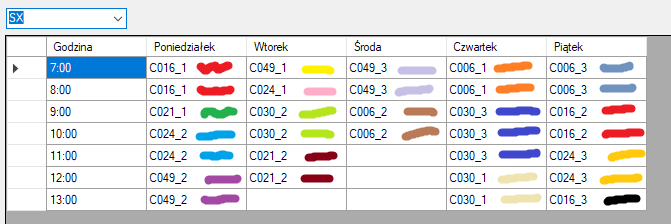
\includegraphics[width=\textwidth] {sx}
	\caption{Najlepszy otrzymany plan zajęć dla najlepszego rozwiązania.}
	\label{fig: sxkopia}
	\end{figure}
	
	\begin{figure}
	\centering
	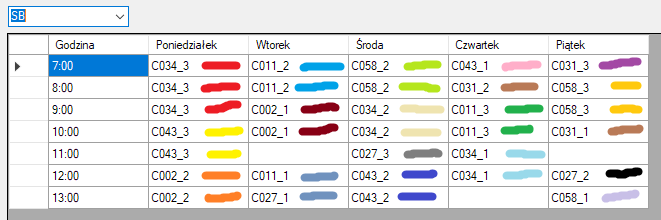
\includegraphics[width=\textwidth] {sb}
	\caption{Najgorszy otrzymany plan zajęć dla najlepszego rozwiązania (2 okienka).}
	\label{fig: sbkopia}
	\end{figure}

Najlepszy wynik otrzymany został dla następujących parametrów wejściowych: liczba iteracji - 1000, długość tabu - 500, rozmiar sąsiedztwa  - 300. Liczba iteracji algorytmu została ustalona biorąc pod uwagę czas pracy programu oraz fakt, że liczba ta zazwyczaj wystarczała, by usunąć wszystkie konflikty z planu zajęć. 

Rozmiar sąsiedztwa również w dużej mierze wpływa na czas pracy algorytmu. Z drugiej strony doświadczenia pokazały, że im większe sąsiedztwo tym mniej iteracji potrzebnych do uzyskania lepszych wyników. Rozmiar 300 to około 5\% całego sąsiedztwa możliwego do przeszukania. Ustawienie algorytmu na przeszukiwanie 100 \% sąsiedztwa, spowodowało by wydłużenie pracy algorytmu dwudziestokrotnie. Ustalony rozmiar jest próbą pogodzenia oczekiwań jak najkrótszego czasu pracy algorytmu i jak najlpeszych wyników.

Długość tabu zmienia całkowicie sposób pracy algorytmu. Ustalenie wartości 500 wynikało z obserwacji wyników jakie dostarczał algorytm oraz wykresów, obrazujących jego pracę. Szczegółowe omówienie wpływu parametru długości Tabu przedstawiono w kolejnym podrozdziale.

\section{Znaczenie parametru długości Tabu.}

